In this chapter we will go through how the installations have been analysed and present the findings.

\section{Systematising the installations}
Over the course of this thesis, my research buddies and I have visited 7 exhibitions from 4 local museums in Oslo. Two of the exhibitions took place at the University of Oslo: department of informatics (ifi), as part of the course Tangible Interaction (IN5470). From these museum visits, we have documented 21 interactive installations that make up the data-set.

\begin{table}[H]
\centering
\begin{tabular}{l | l| l}
\textbf{Type} & \textbf{Name} & \textbf{Museum}\\
\hline
Exhibition & Vi står i det nå & Klimahuset \\
Exhibition & I/O (In Oslo) & Atelier Nord\\
Exhibition & Shadows & MUNCH\\
Exhibition & Poison & MUNCH \\
Exhibition & Input/Output & Teknisk Museum \\
Exhibition & Slow Design: reveal & ifi \\
Exhibition & Haptic Interaction & ifi \\
\end{tabular}
\caption{Exhibitions}
\label{tab:abc}
\end{table}

\begin{table}[H]
\centering
\begin{tabular}{l | l}
\textbf{Exhibition} & \textbf{Installation}\\
\hline
I/O (In Oslo) & I/O (In Oslo)\\
Input/Output & Input/Output  \\
Slow Design & Qi \\
Slow Design & Memento Mori \\
Slow Design & Presence in existence \\
Haptic Interaction & The Maze \\
Haptic Interaction & Black Horizon \\
Haptic Interaction & The unfair fun fair \\
Vi står i det nå & Crank lever \\
Vi står i det nå & Rotating disc \\
Vi står i det nå & Solutions \\
Vi står i det nå & Video theatre \\
MUNCH & Poison  \\
MUNCH & Shadows -- Paint like Munch \\
MUNCH & Shadows -- Resting sofa chair  \\
MUNCH & Shadows -- Camera \\
MUNCH & Shadows -- Edvard M. paints your portrait  \\
MUNCH & Shadows -- Radio \\
MUNCH & Shadows -- Telephone  \\
MUNCH & Shadows -- Suitcases  \\
MUNCH & Shadows -- Housekeeper  \\
\end{tabular}
\caption{Installations}
\label{tab:abc}
\end{table}


\begin{comment}
\begin{table}[h]
\centering
\begin{tabular}{l | l| l}
\textbf{Type} & \textbf{Name} & \textbf{Museum}\\
\hline
Literature review & Museums and Sustainability & \\
Prototyping & The relationship between human and nature \\
Presentation & Exploring input through plants & Klimahuset\\
Exhibition & Liquid Life & Kistefoss \\
Observation & Climate Dialogue w/ 2 school classes & Klimahuset\\
Interview & Concept Developer & MUNCH\\
\end{tabular}
\caption{Other fieldwork}
\label{tab:abc}
\end{table}
\end{comment}

\section{Application of theoretical framework}
In this section we will see how the analytical tool have been put to use. To start the shaping of the framework-triangle, it made the most sense to me to create one table for each theory; \emph{Hybrid place, Dialogic place and sense-making}. This way we could quantify the data, as one way of comparing the principles and see how they play together. The installations are listed in the column to the right(x-axis), and the principles/ and dimensions in rows (y-axis), see reference picture in figure 9.1, or 9.2. This way we could see how applicable the theories (principles/ and dimensions) are for the dataset, and hopefully it would open for seeing connections across/ between the theories as well; "The bigger picture". Figure 9.1 illustrates how each theory contribute to the understanding of meaningfulness. The lines represents what we strive to find; dialogic relations between visitor and installation, and objectifying meaningfulness as a quality that you can design for.

\begin{figure}[H]
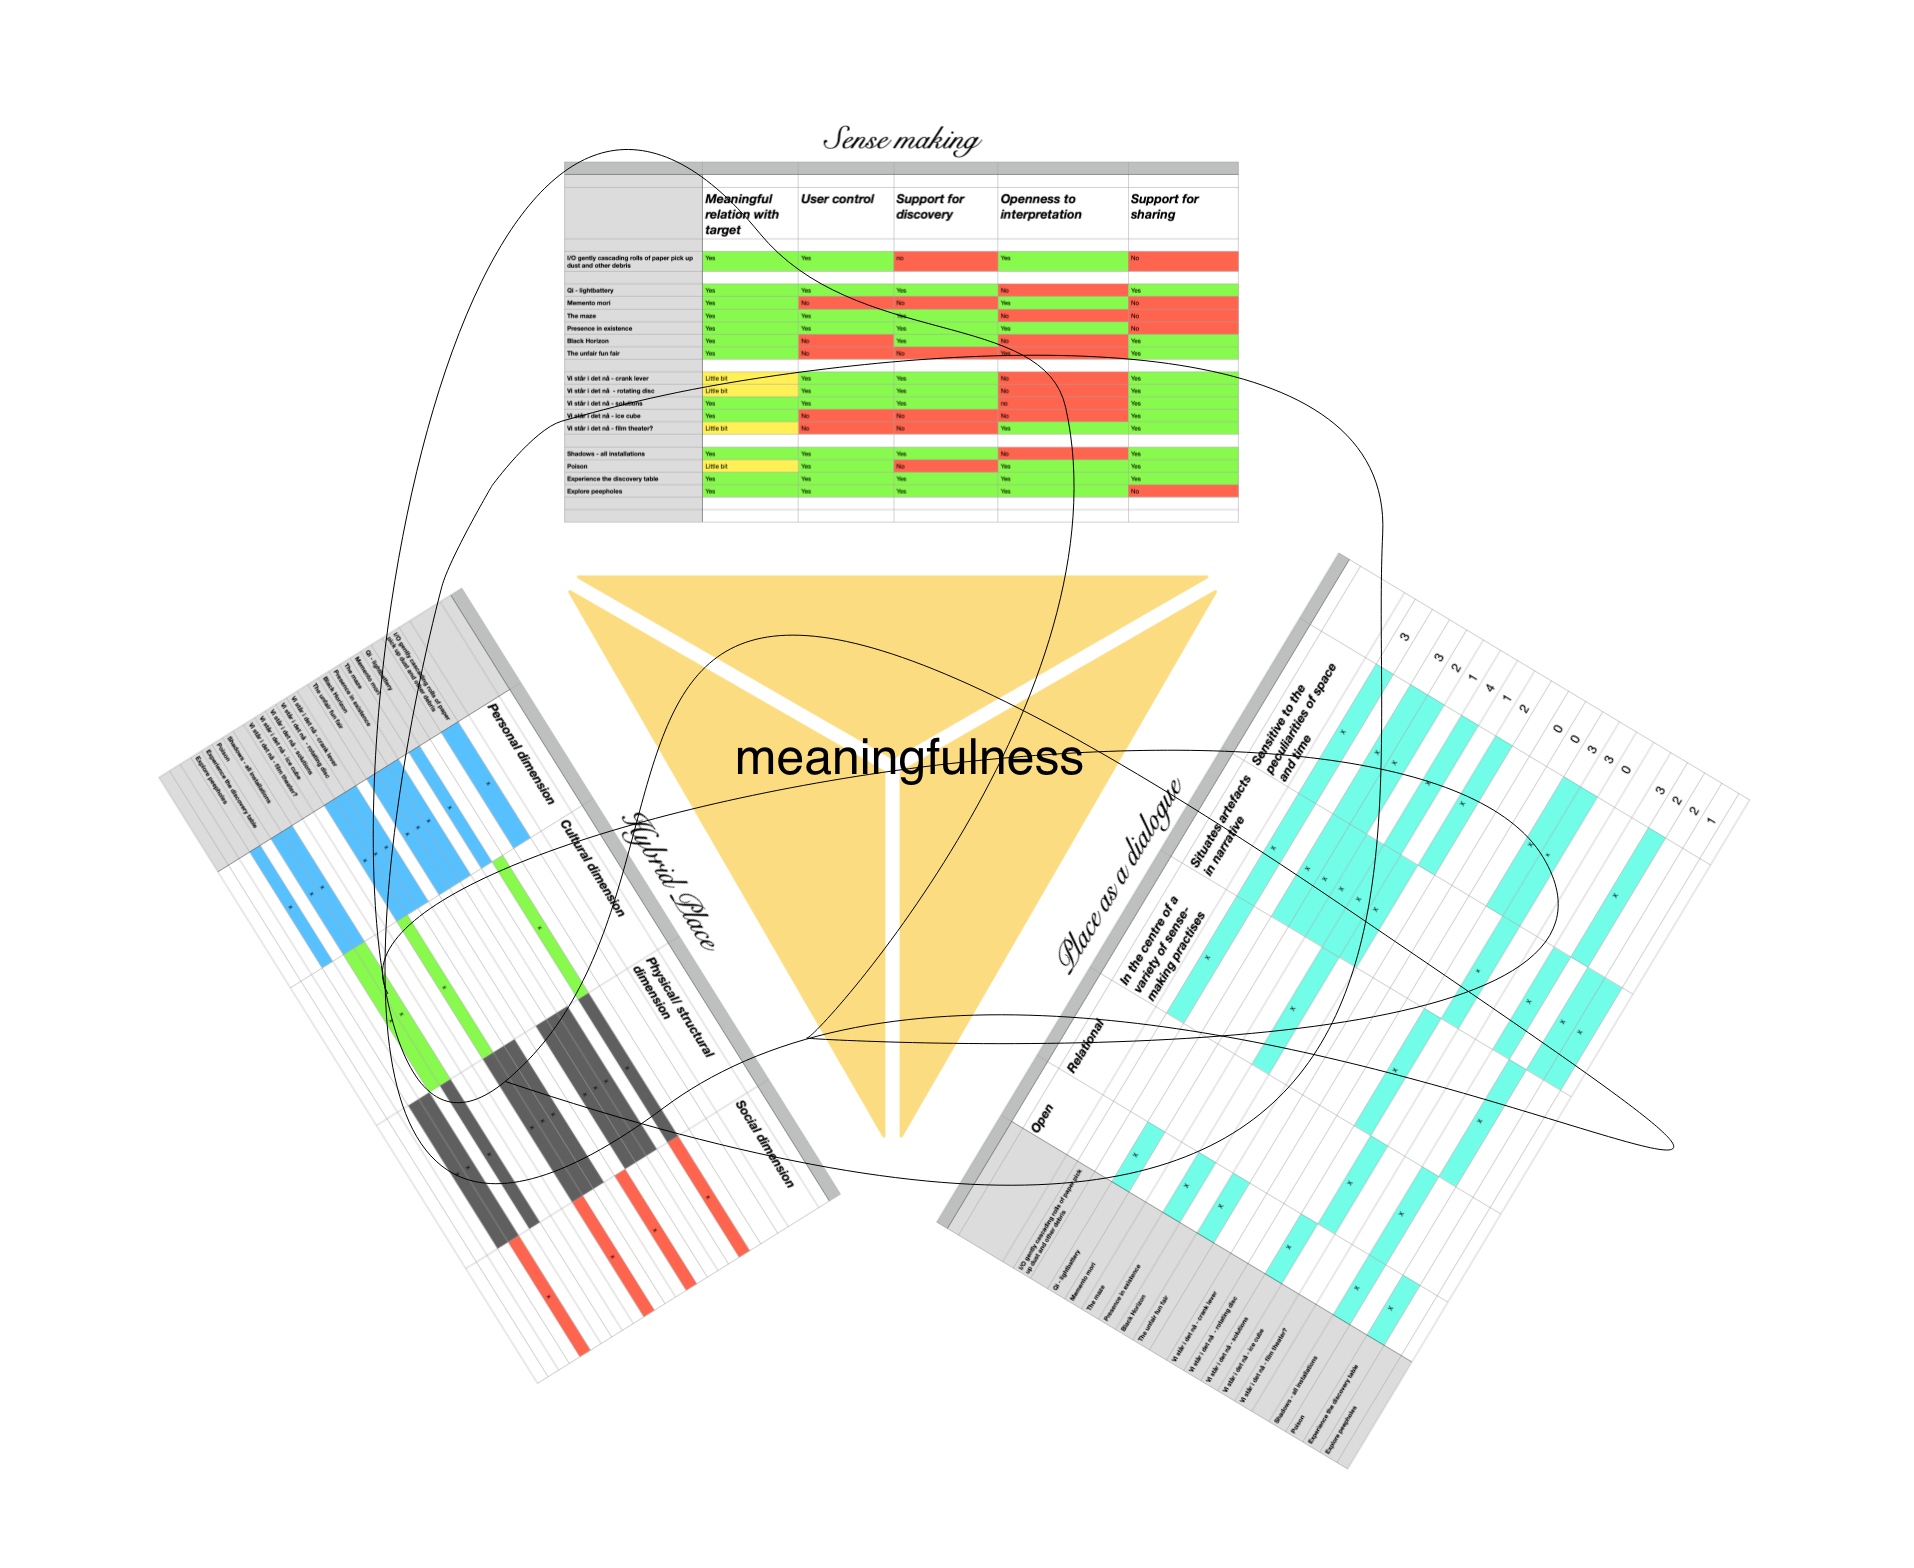
\includegraphics[width=14cm]{pictures/analysis/table_triangle.png}
\caption{Illustrates how each theory contribute to the understanding of meaningfulness. The lines represents what we strive to find; dialogic relations between visitor and installation, and objectifying meaningfulness as a quality that you can design for}
\end{figure}

The plotting of the tables are based upon the written experience accounts and my subjective intuition consisting of both my memory and take-away of the installation. 

\textbf{Hybrid place table}

Seeing that all written experience accounts are based on the hybrid place dimensions, this table was quite straight-forward to work with. What we see from this table is 

Wanting to get a place-centred understanding of the installations, one whole side/edge of the triangle-framework I present are built upon the four dimensions presented by \autocite{hybridplace_ciolfi}; the \emph{personal}, \emph{cultural}, \emph{physical/structural}, and \emph{social} dimension, accounted for in chapter 3.



\textbf{place as dialogue qualities}

Wanting to get a better understanding of the visitor experience with attention to the sensory transactions and the way the experience transform in the telling (what is the things you remember), I utilise \autocite{spaceplace_ciolfi} "dialogical ontology", or as I call it, the list of place-related qualities. 

\textbf{Dissemination}
Then, the sense-making strategies make up



\begin{figure}[H]
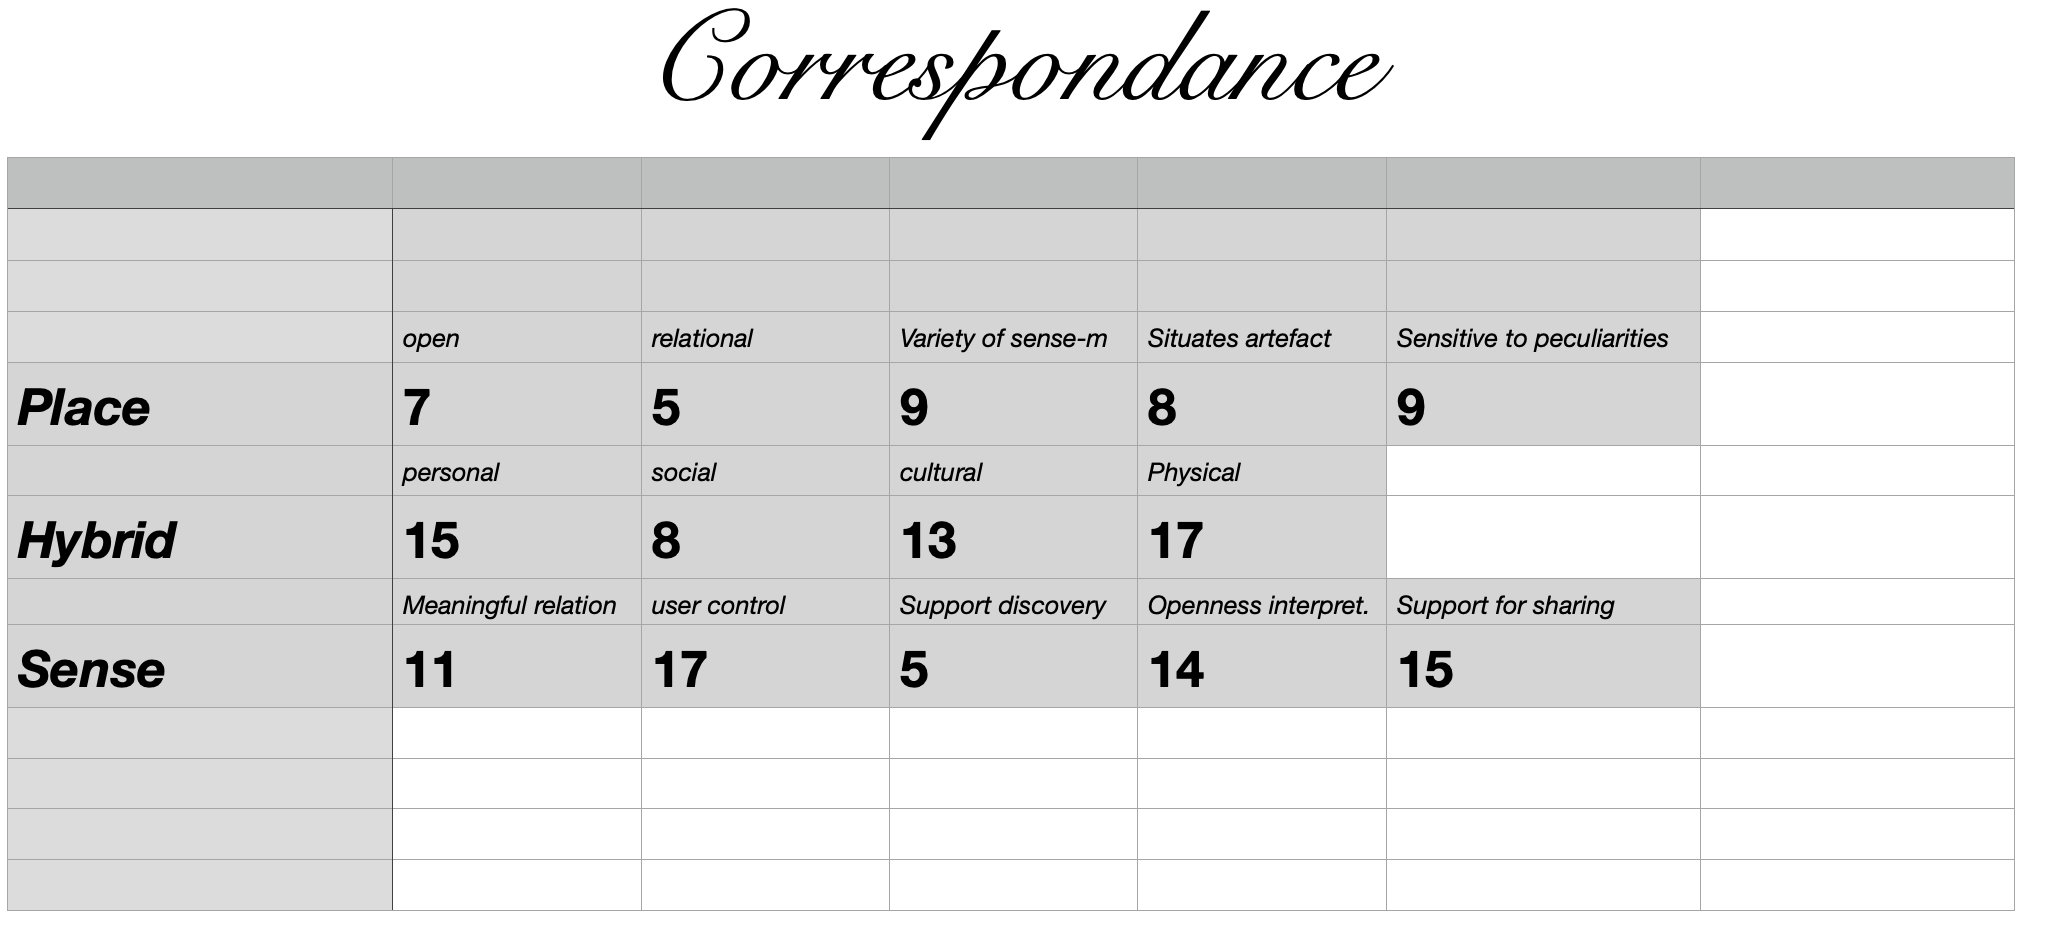
\includegraphics[width=12.5cm]{pictures/analysis/correspondance.png}
\caption{Correspondence table}
\centering 
\end{figure}

\begin{figure}[H]
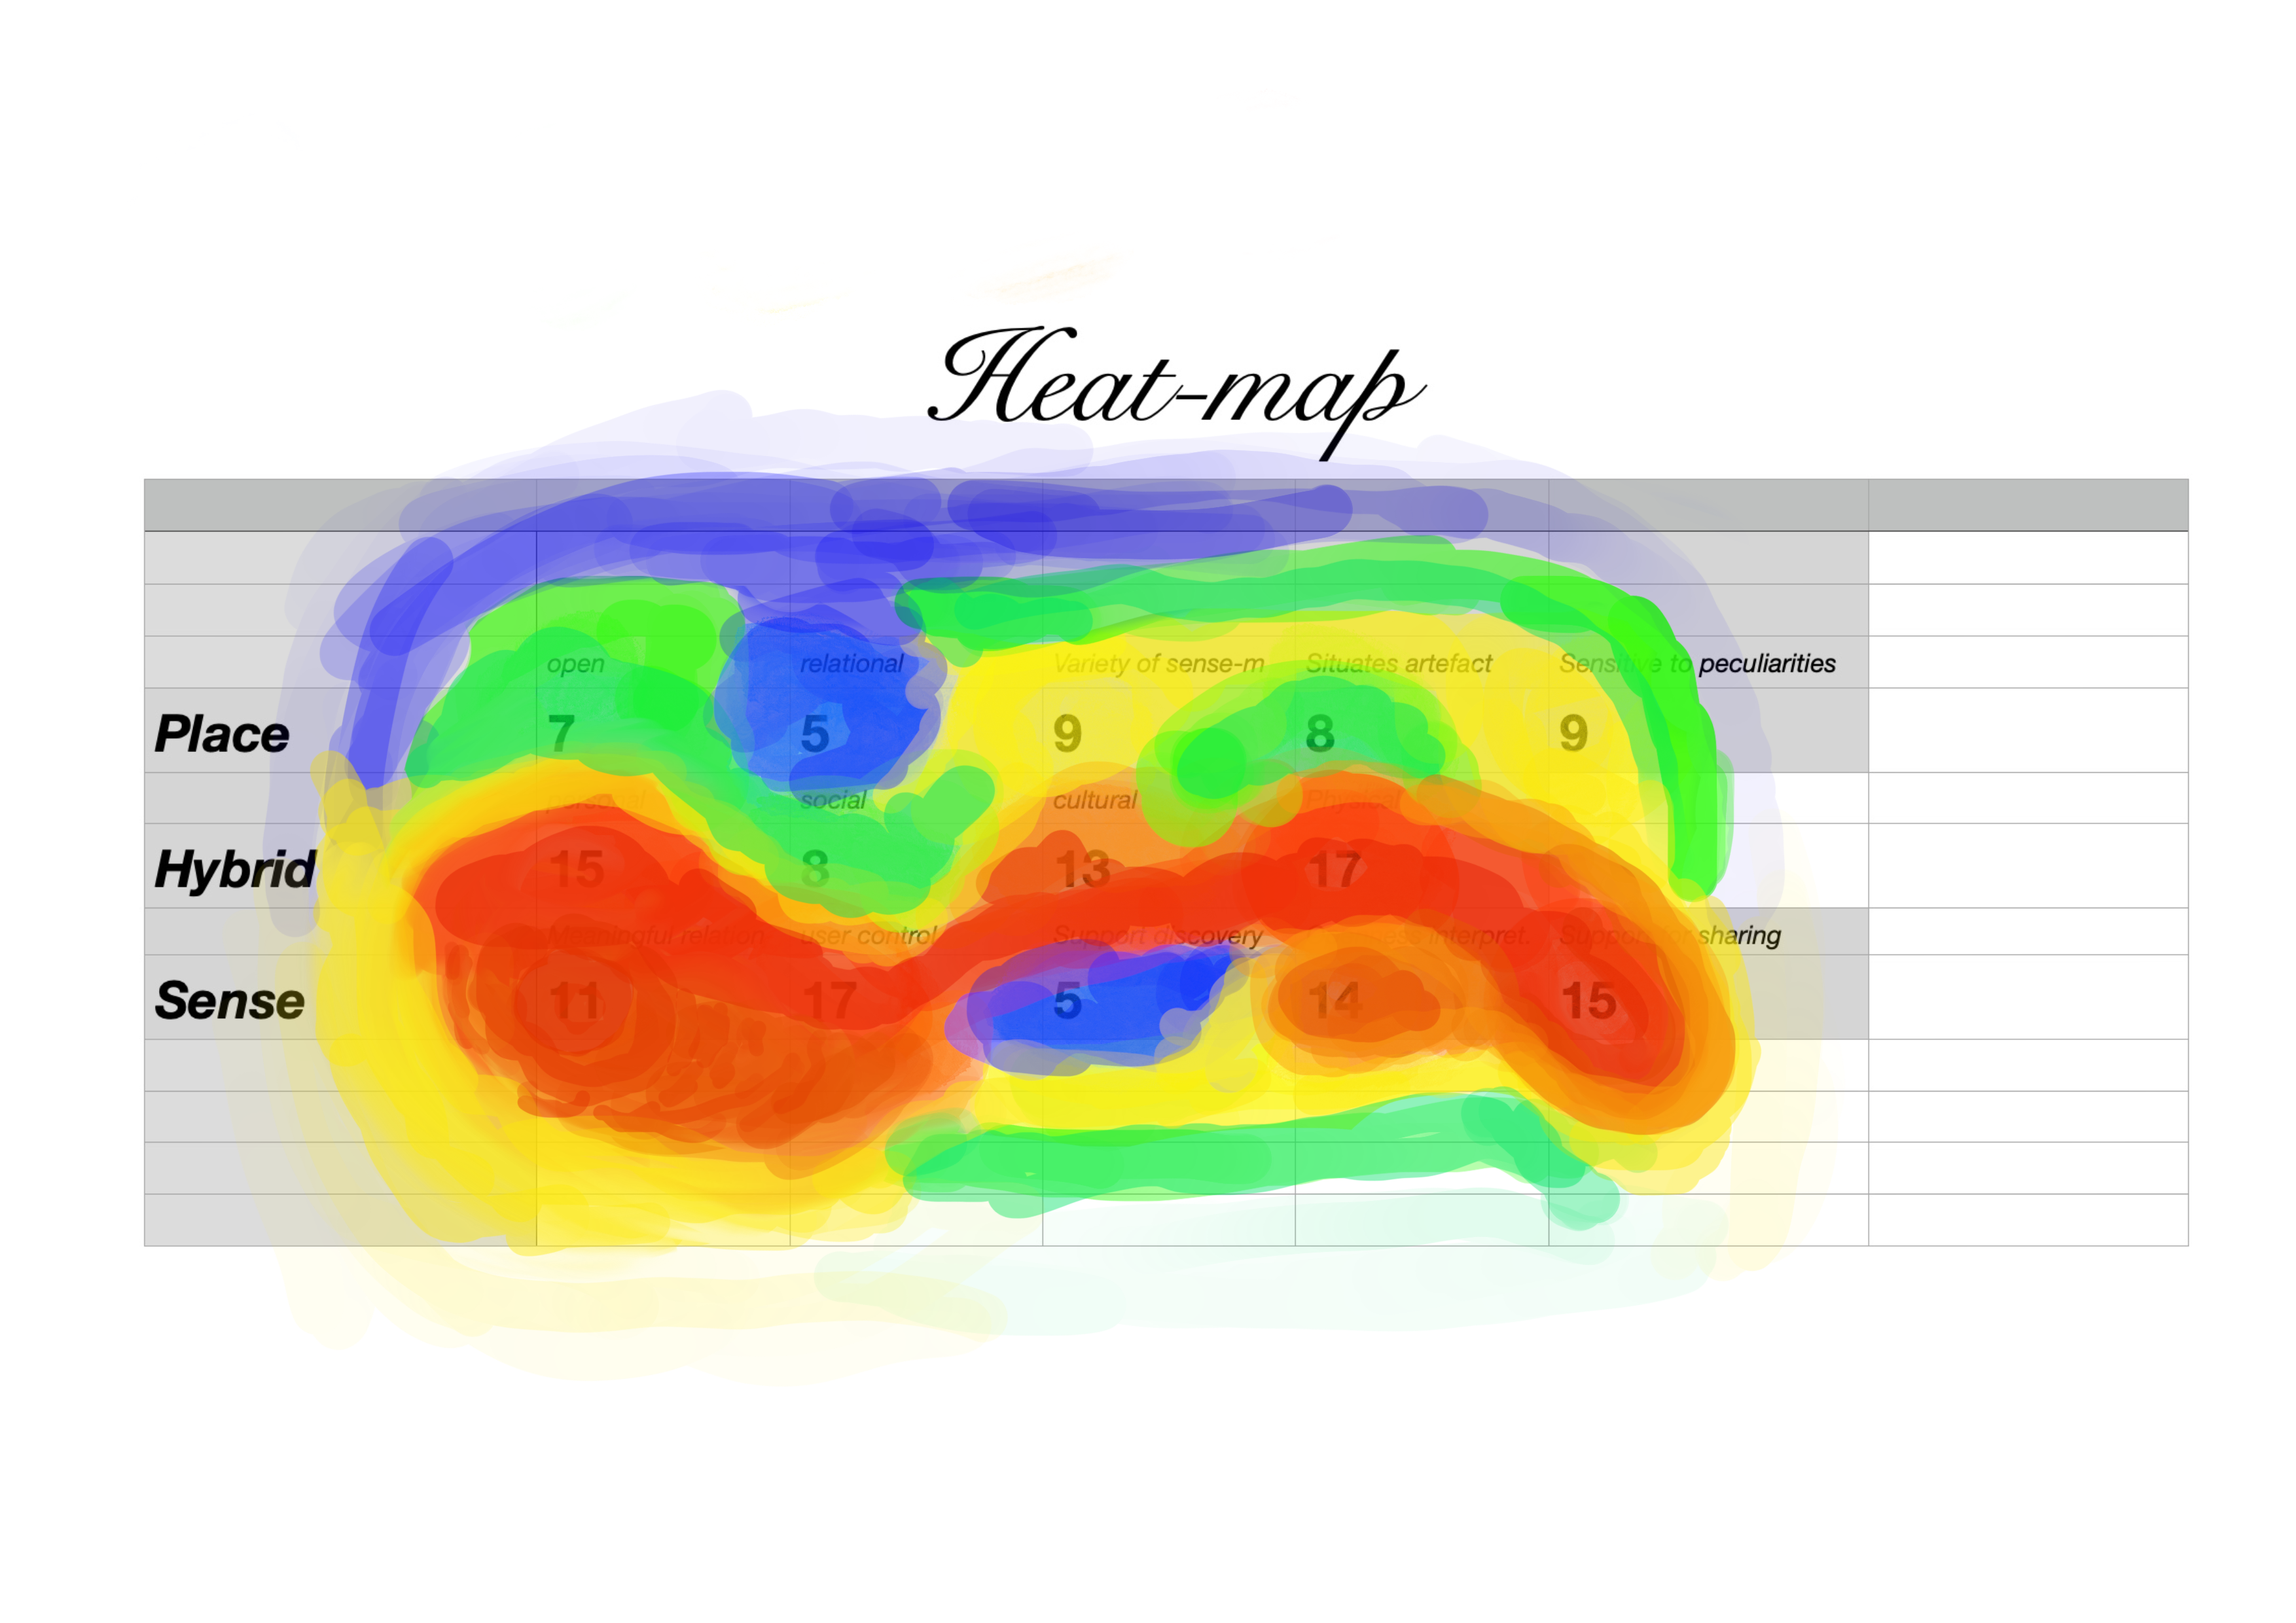
\includegraphics[width=12.5cm]{pictures/analysis/heatmap.png}
\caption{Heat-map}
\centering 
\end{figure}

\subsection{Hybrid Place}
\begin{figure}[H]
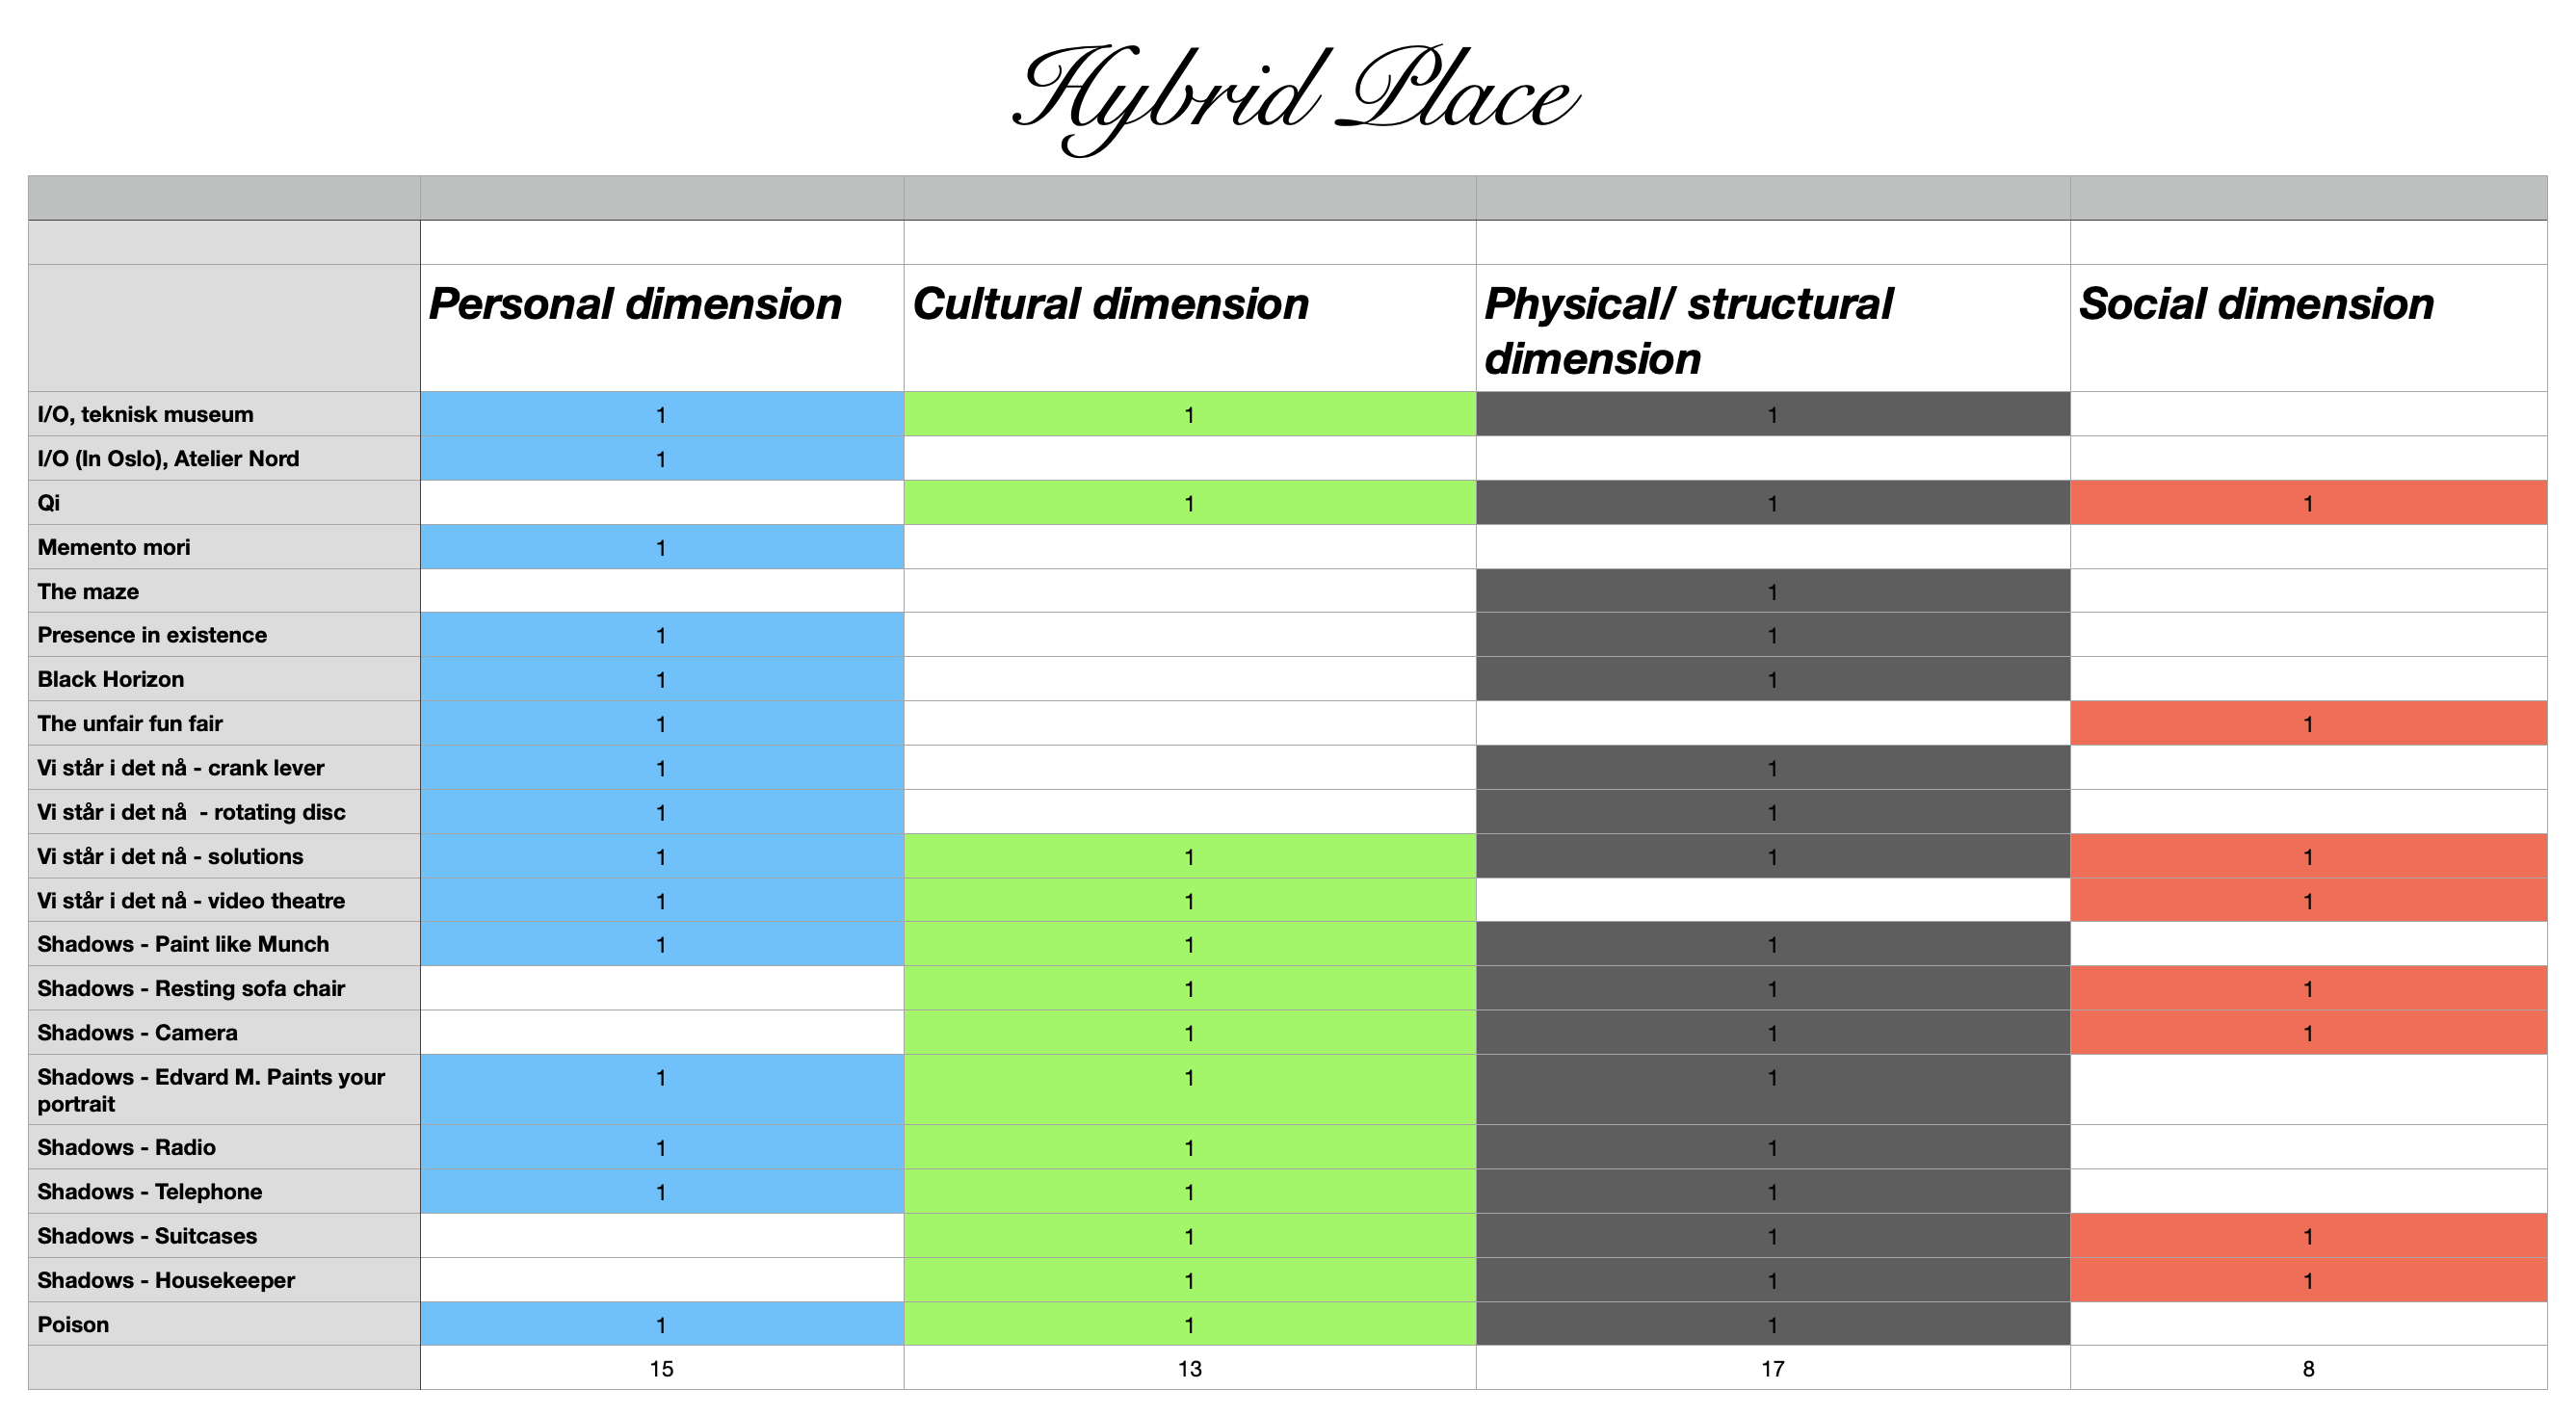
\includegraphics[width=20cm, angle=90]{pictures/analysis/hybrid.png}
\caption{Hybrid Place table}
\centering 
\end{figure}

\begin{figure}[H]
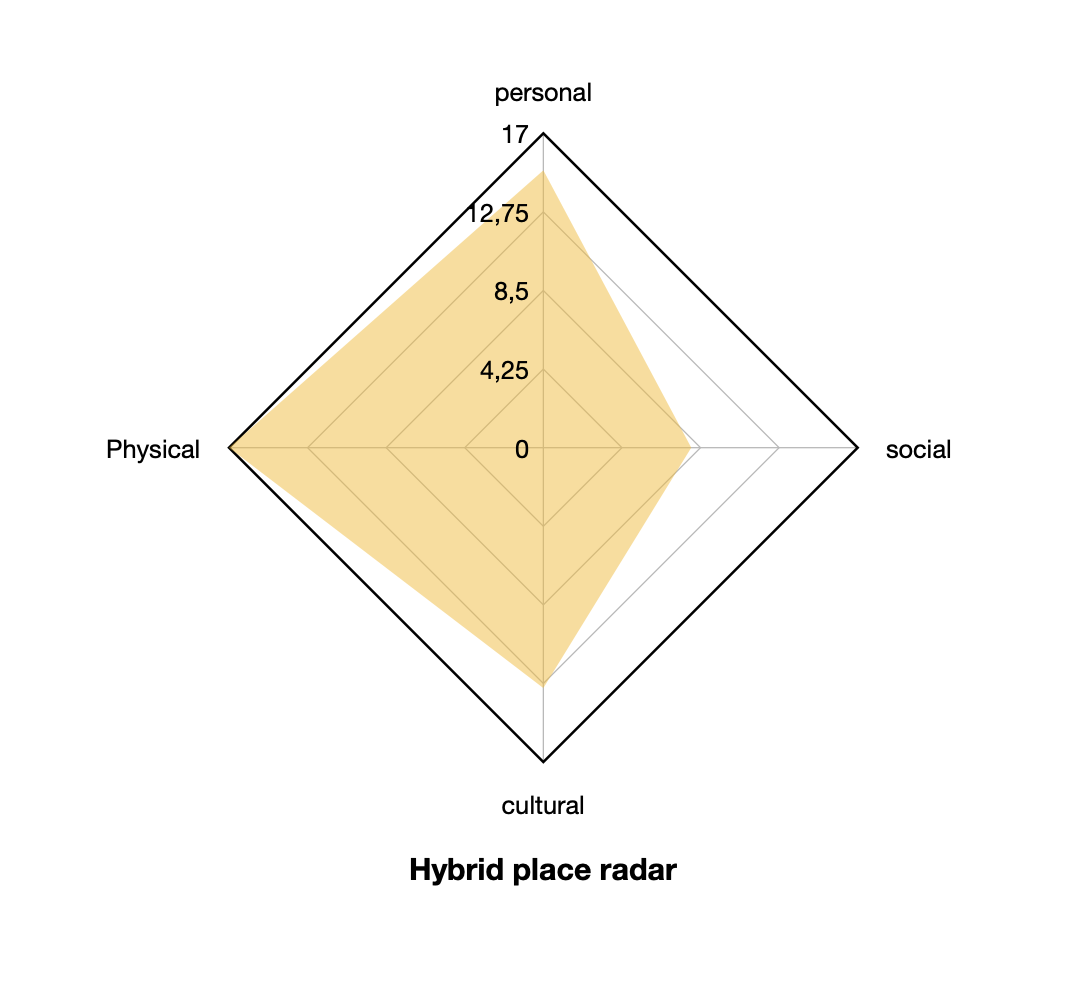
\includegraphics[width=12.5cm]{pictures/analysis/hybrid_radar.png}
\caption{Hybrid Place table}
\centering 
\end{figure}

\subsection{Place as a dialogue}
\begin{figure}[H]
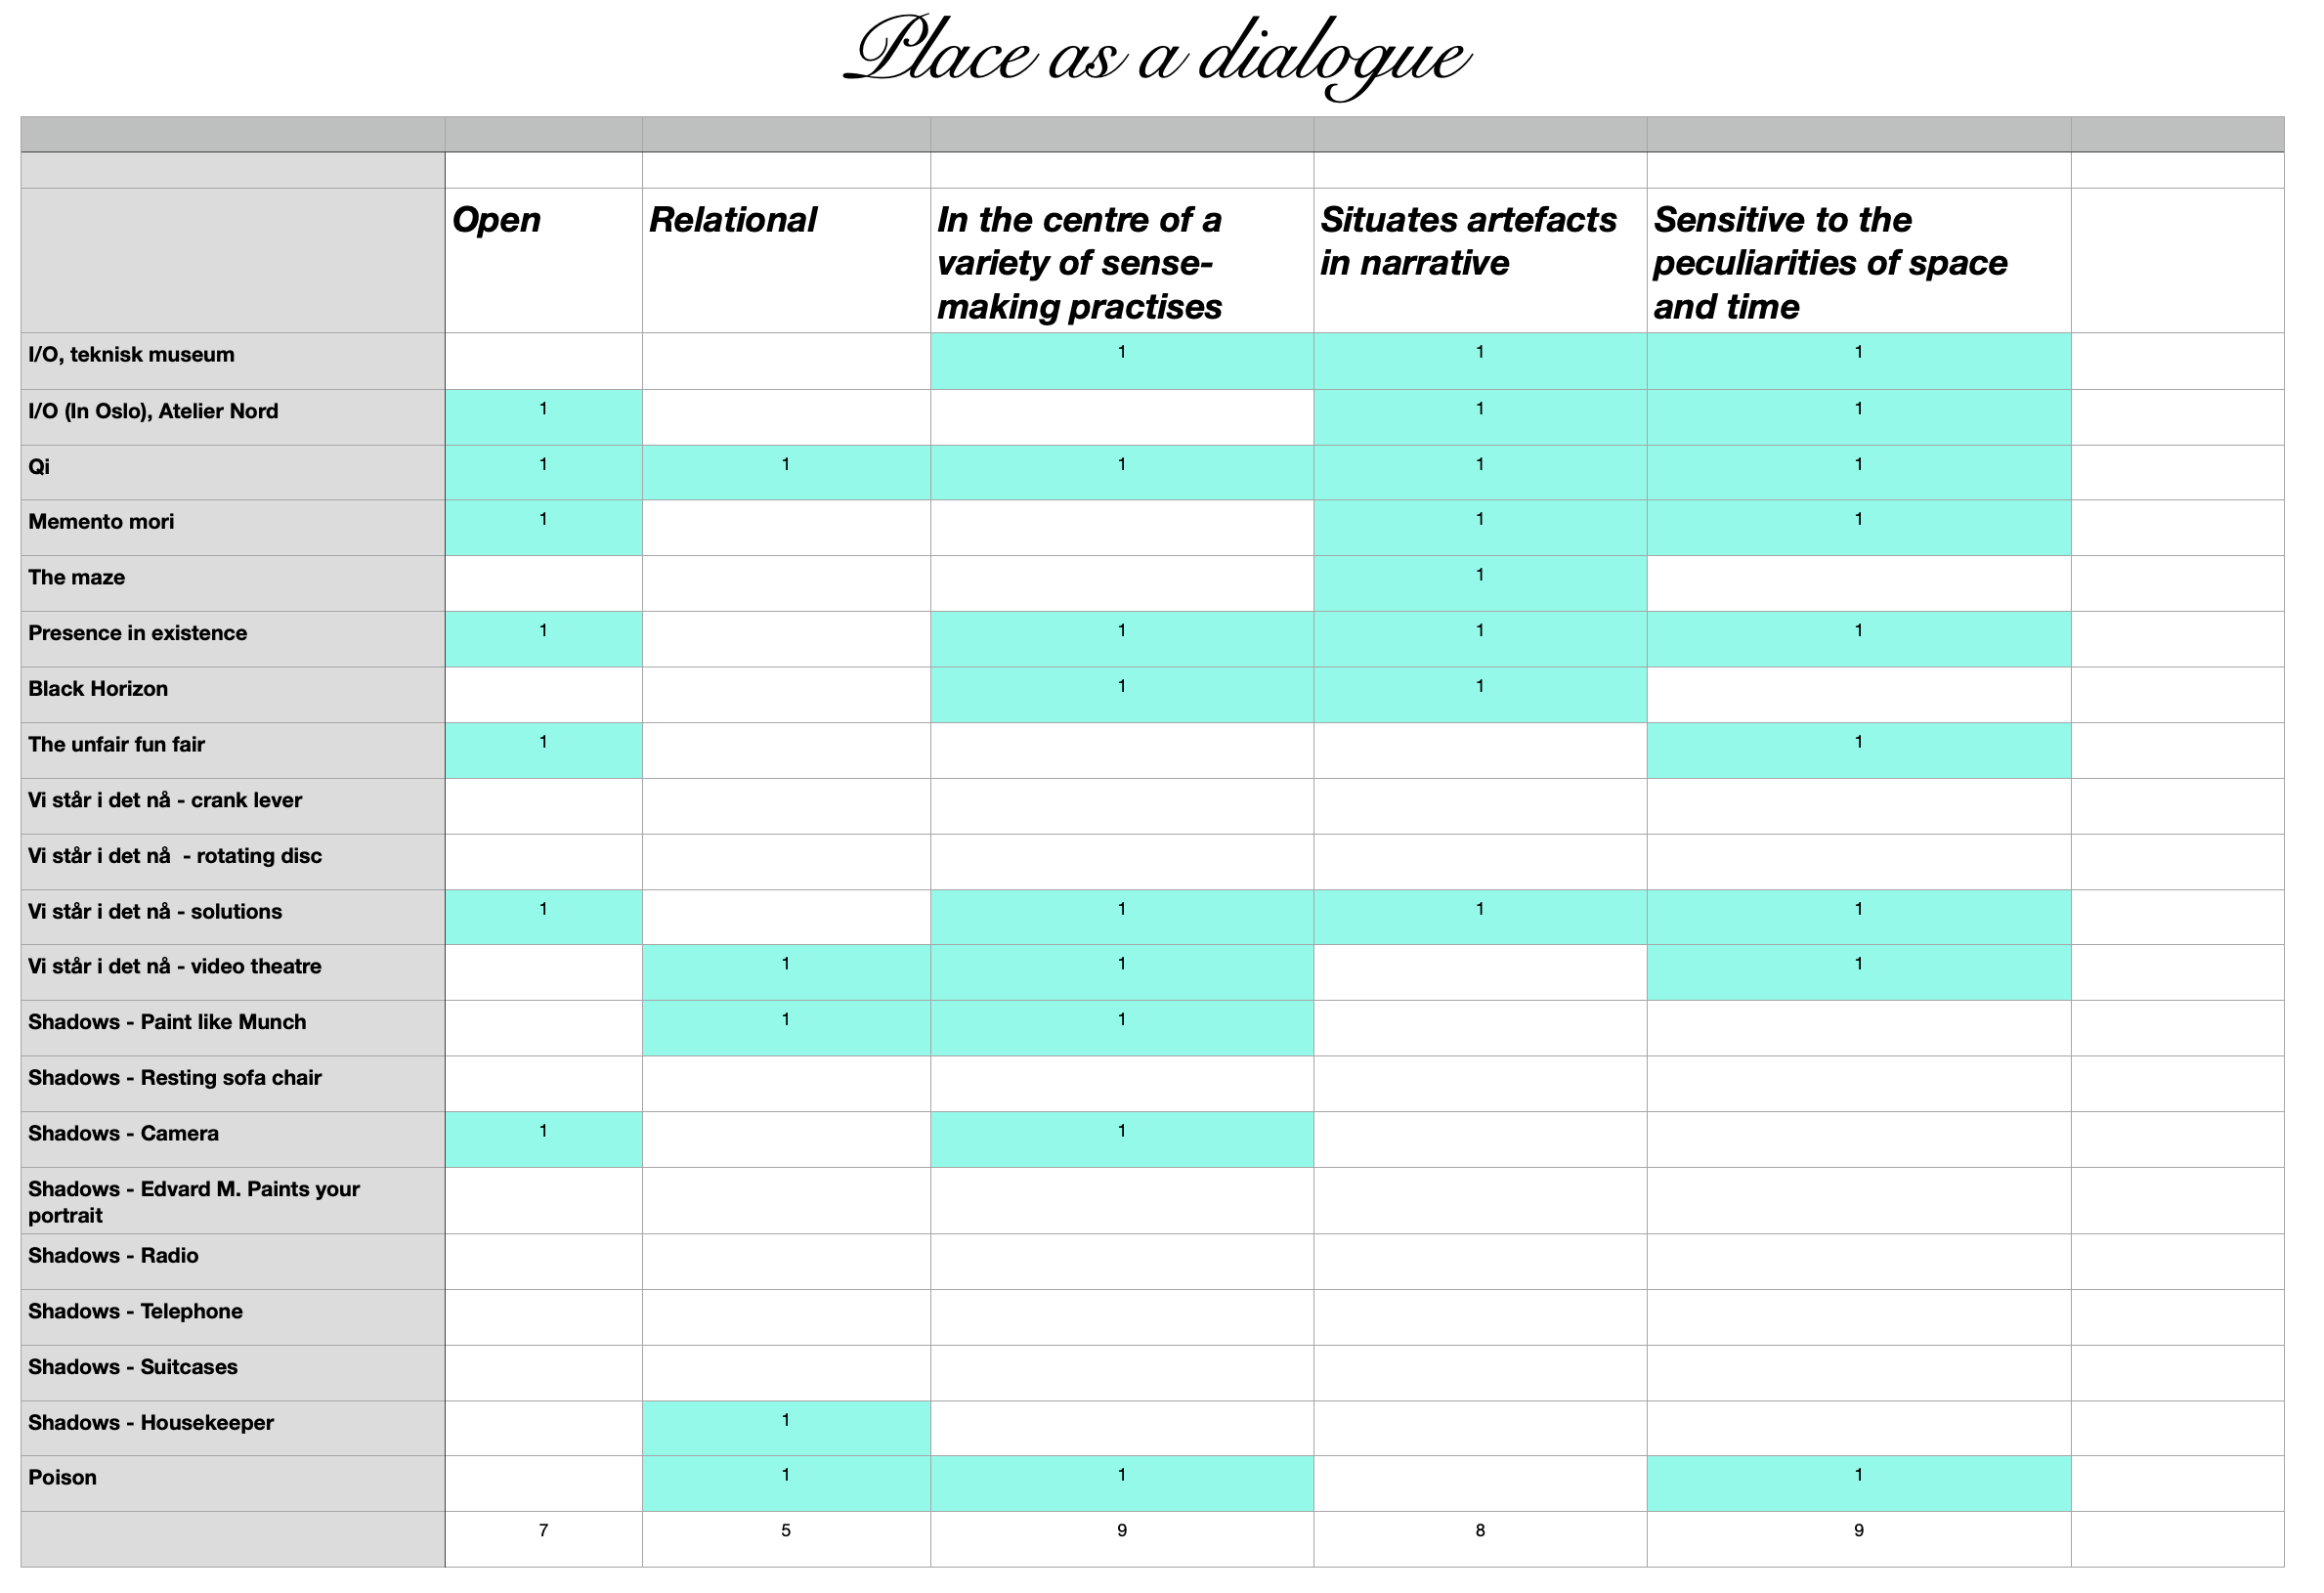
\includegraphics[width=20cm, angle=90]{pictures/analysis/place.png}
\caption{Place as a dialogue table}
\centering 
\end{figure}

\begin{figure}[H]
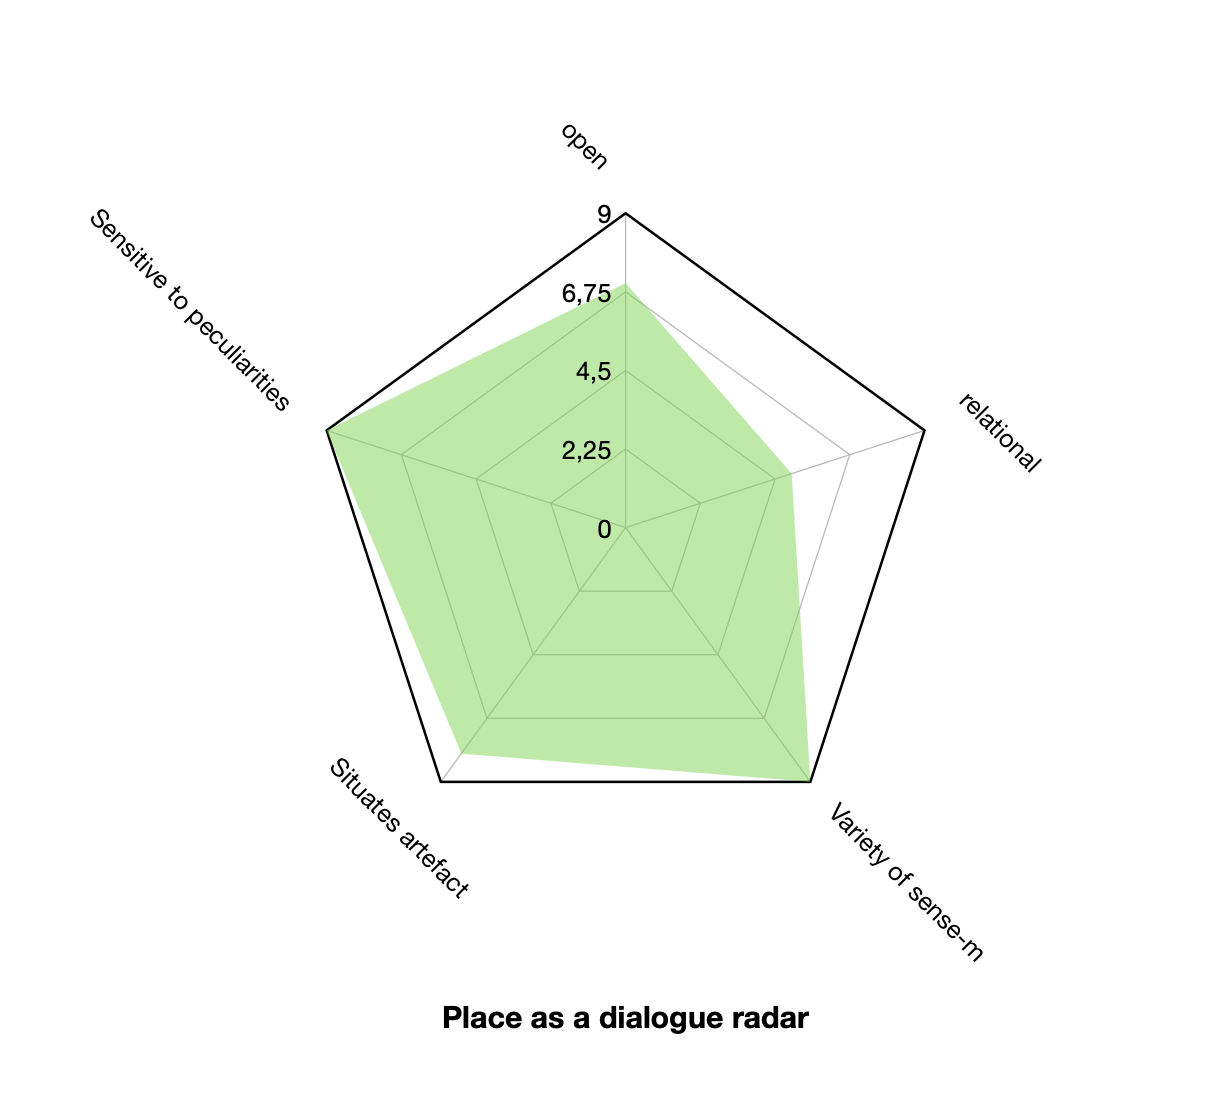
\includegraphics[width=12.5cm]{pictures/analysis/place_radar.png}
\caption{Place as a dialogue radar}
\centering 
\end{figure}

\subsection{Sense-making strategies}
\begin{figure}[H]
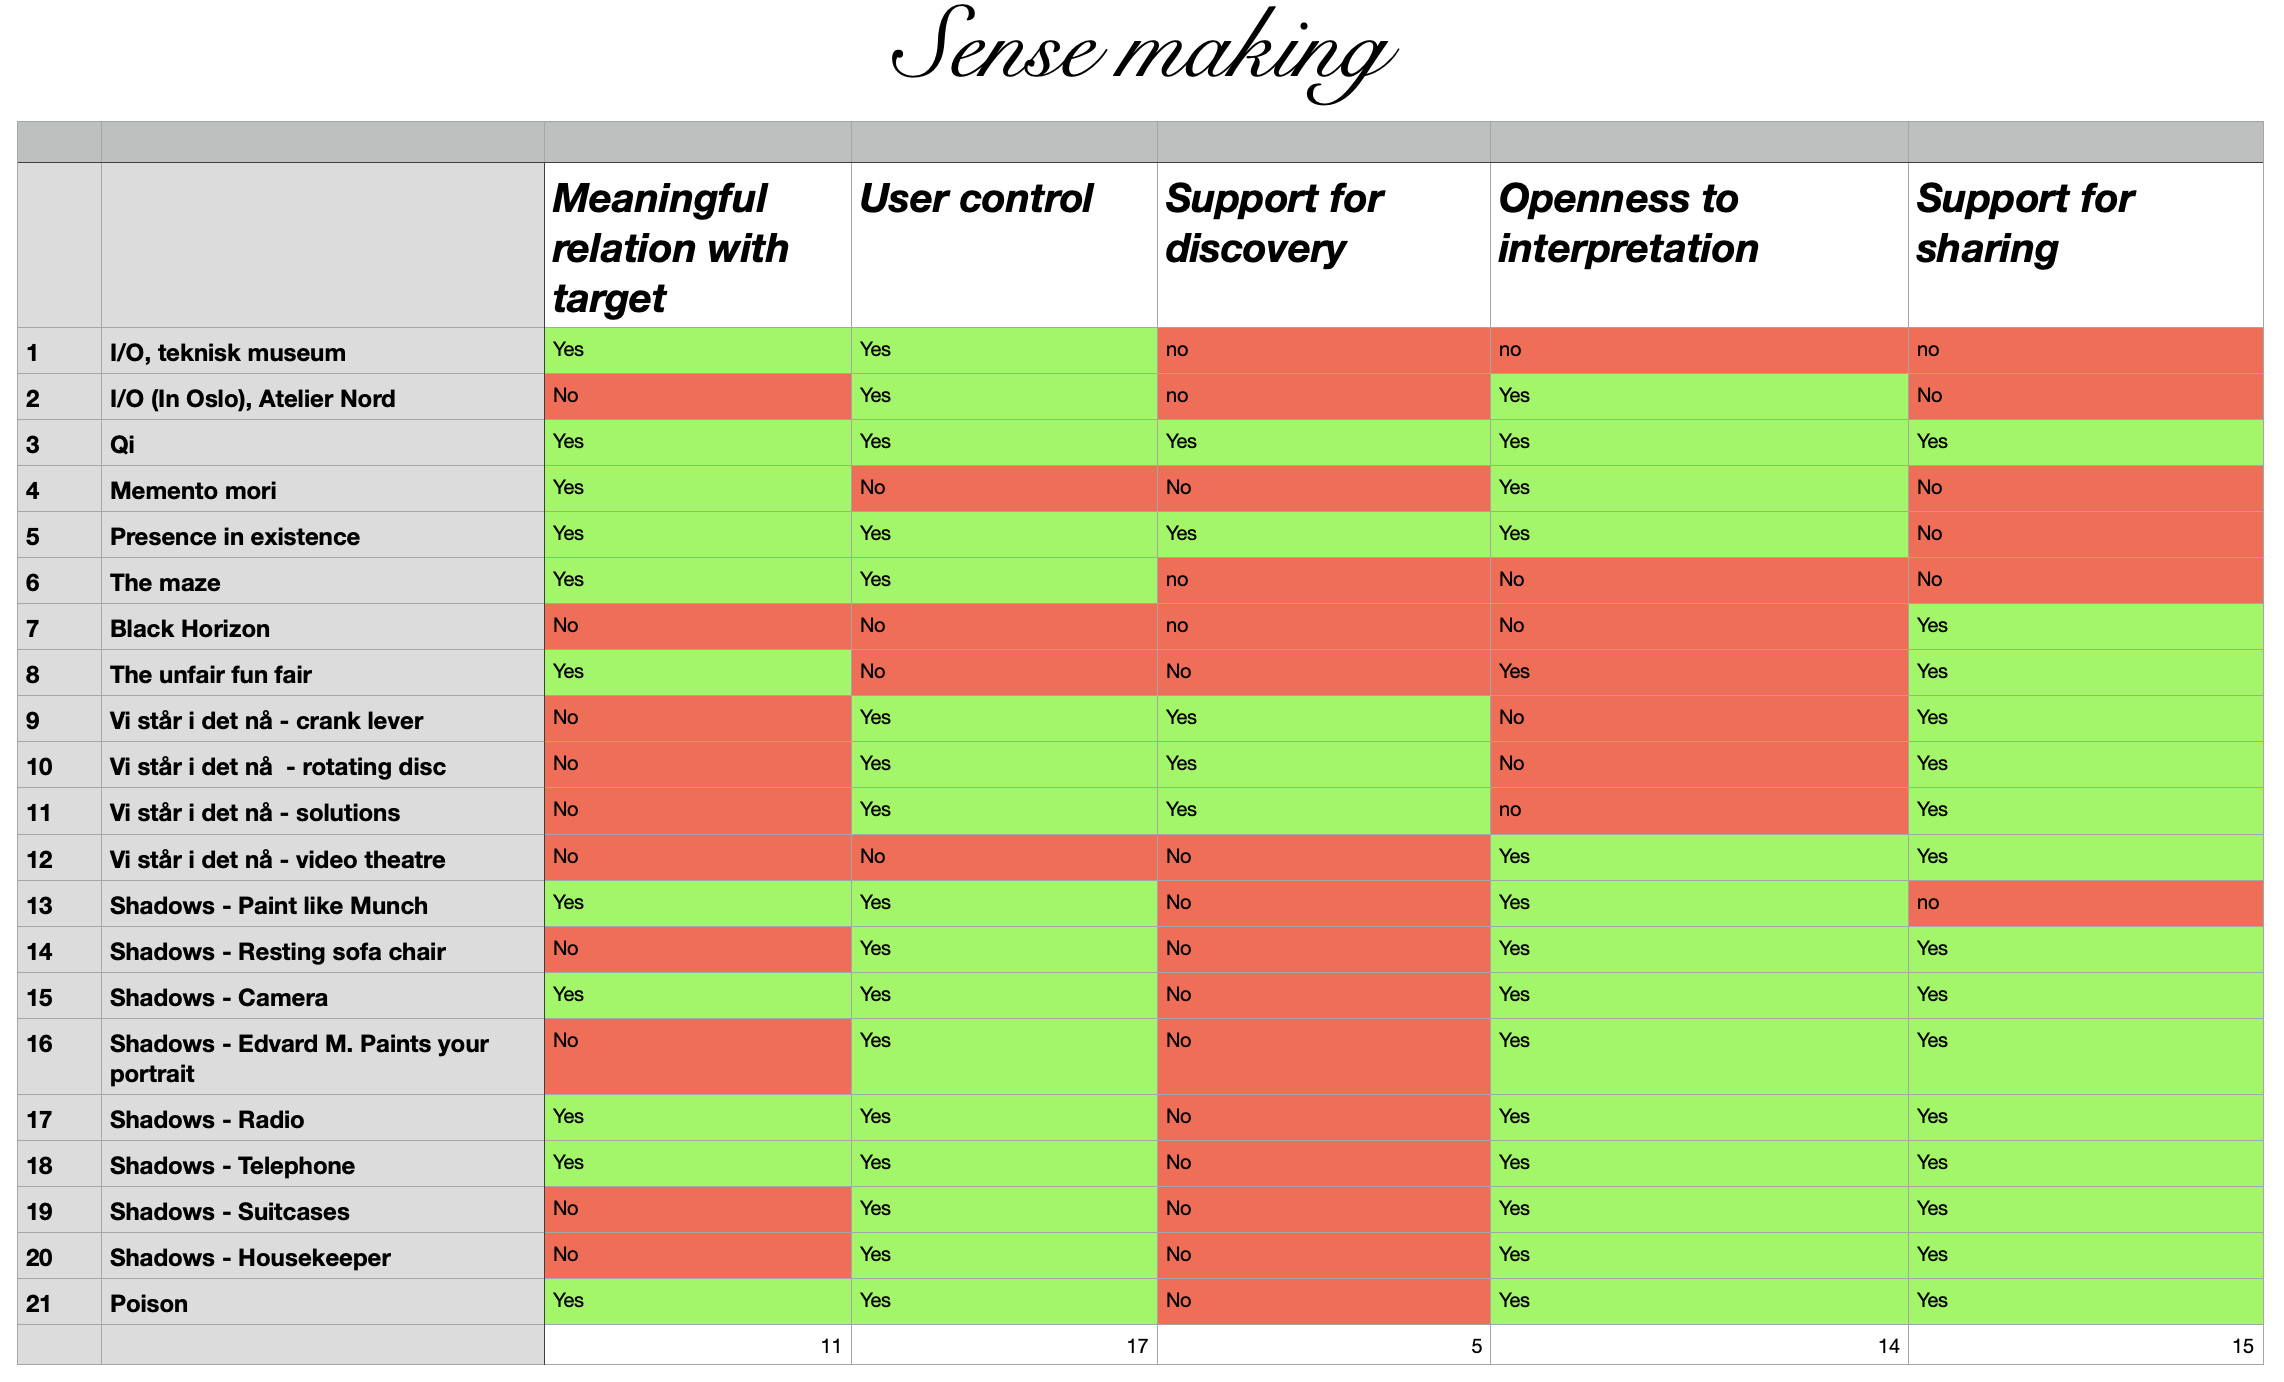
\includegraphics[width=20cm, angle=90]{pictures/analysis/sense.png}
\caption{Sense-making strategies table}
\centering 
\end{figure}

\begin{figure}[H]
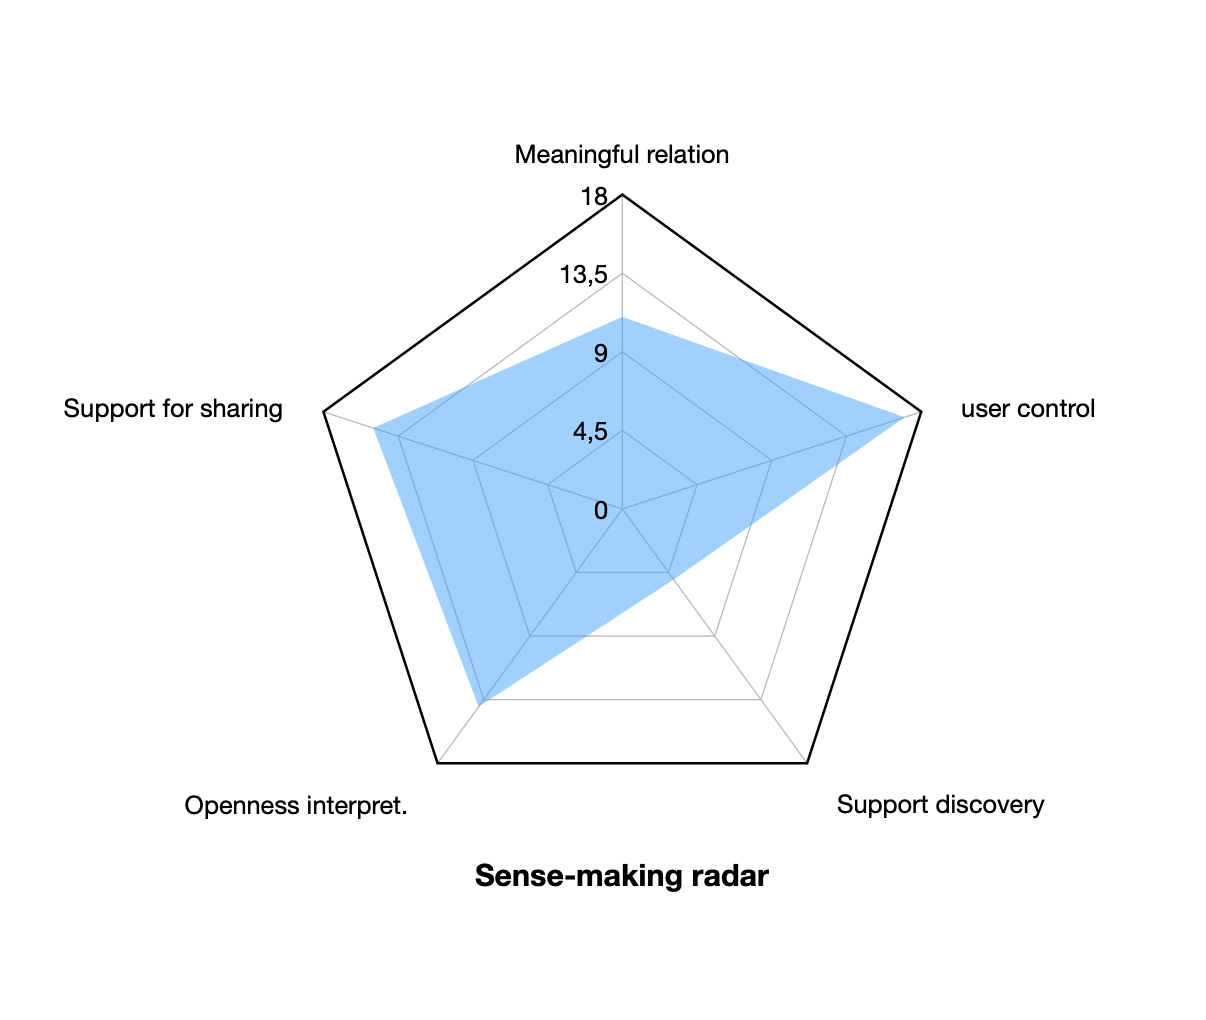
\includegraphics[width=12.5cm]{pictures/analysis/sense_radar.png}
\caption{Sense-making radar}
\centering 
\end{figure}


\section{Findings}

In my attempt to answer how one can design meaningful interactive experiences in a museum space that addresses sustainability, I have accounted for three theories I base my understanding of meaningfulness on; \emph{Hybrid place, place as a dialogue} and \emph{Sense-making strategies}. (My notion is that), together they form the basis to identify meaningful relations between visitor, installation and the museum. 


I made one table for each theory, where the frameworks's principles/ and dimensions formed the columns and the 22 different installations the rows. I then went through each installation and plotted in whether or not the installation fulfilled the principle/ dimension. Categorising it this way opened up for looking at the dataset in correlation with each theory separately, making it possible to see overall trends in the dataset according to the theories. Another respective theory from a birds-eye, holistic, perspective, but it will also work as a quick-reference guide for the second analysis iteration when I'm trying to merge the three theories and/ or finding new relationships between the data across the theories.

The categorisation of the data is highly subjective, but theoretically grounded, based on my personal experience with- and interpretation of the installations and knowledge of the museum institution the installation was part of. I have also chosen to merge all the Munch - \emph{Shadows} installations as one, because they are a part of the same exhibition and do not differ in their interactive qualities. Because of this, the dataset used for this analysis shrinked from 22 to 16. This choice of merging the \emph{Shadows} installations was made in the process of fitting the installations into the theory's principles/ dimensions, when I saw that they all checked the same boxes. 


After mapping the installations in the tables, it opened up for crunching the first numbers. In this iteration I want to see the dataset from a holistic view. Abstracting from the details and seeing how the installations map up in the bigger picture. To do this I needed a diagram that could compare the different principles up against eachother. I chose to create radar charts to do this, and made a radar chart for each theory. 


\emph{"Findings"}
\par

What I have learned by looking at the radar charts so far is how the different theories fulfill, or complement eachother. The way I have gone forward in looking at the radar charts is as following:
\par I'll start by looking at the hybrid place radar chart, noticing how the personal and physical dimension is fulfilled, while the social and cultural dimension is very little fulfilled. What does this mean? According to the Norwegian museum policy strategic thinking, it is wanted that museums transition from the personal dimension to the more social and cultural dimension. The fact that installations in my analysis shows presence in the physical dimension is positive, in terms of enabling the personal dimension, experience-wise, to involve more tangible or at least dynamic experiences in the museum space.
\par Then, if we shift focus for a second to look into the sense-making radar chart, we see that one of the corners that is fulfilled by almost all installations in this analysis - support for sharing is fulfilled. How come, that even though the social dimension is not fulfilled while almost all installations, in terms of sense-making have good support for sharing? 

\par Then again, we can look at what dialogic qualities the installations turns out to have little "relationalness", which is a dialogic principle/ quality that involves the Docents in the museum for example, or relational qualitites.


\section{Findings}
Because I use theory as an analytical tool, and perhaps use Schön and Wiggins, 


\begin{table}[h]
\centering
\begin{tabular}{l | l}
\textbf{Exhibition} & \textbf{Pattern}\\
\hline
I/O Yuko Mohri & visitors assimilate each-others behaviour \\
Poison & immersiveness in experience

\end{tabular}
\caption{Findings table}
\label{tab:abc}
\end{table}

Pattern from Yuko Mohri:


- Visitors influence eachothers visits. They "acquire" the way we are, and they make us see things we did not see at first. Munch concept developer is also talking about this!

